\section{Thermal Cutoff}

\begin{multicols}{2}

\begin{figure}[H]
\centering
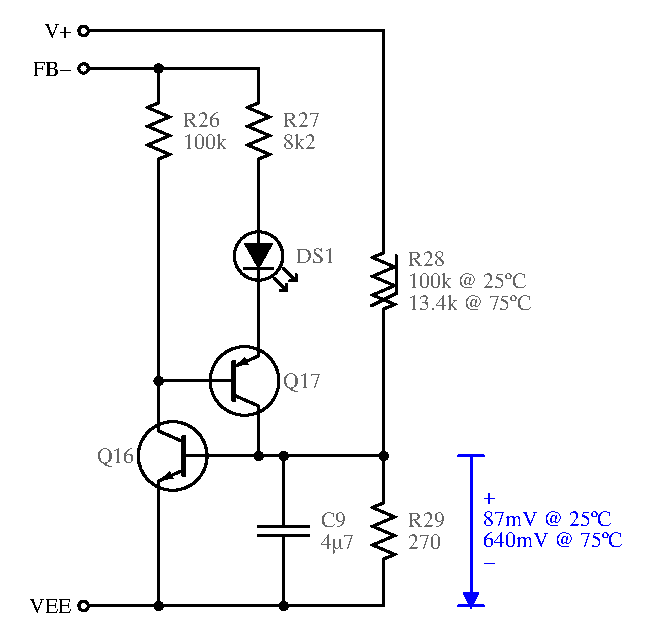
\includegraphics[width=3in]{sch/thermal}
\caption{Thermal cutoff sub-schematic}
\label{fig:thermal}
\end{figure}

The thermal cutoff circuit almost entirely comprises a simulated thyristor,
made from a pair of bipolar transistors.

\begin{figure}[H]
\centering
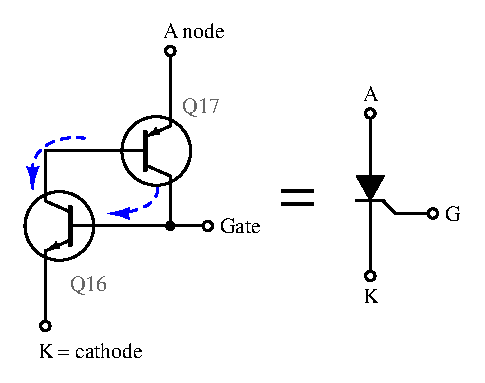
\includegraphics[width=\columnwidth]{sch/thy}
\caption{Simulated thyristor}
\label{fig:thy}
\end{figure}

\subsubsection{Thyristor}

A true thyristor is a device related to the bipolar transistor, made from
four alternating semiconductor layers, P-N-P-N, rather than three.
Unlike the bipolar transistor, it is \emph{bistable}. This means it has a
memory effect --- it can be either `on' or `off', and when put into one of
those states, it will remain there until switched again.

Most thyristors are \emph{silicon controlled rectifiers}, or SCRs.
The SCR's symbol looks like a diode with an extra lead, the \emph{gate}.
In its startup position, with the gate voltage near the cathode voltage, it
does not conduct in either direction. When the gate is activated like the base
of a bipolar transistor, the thyristor begins to act like a diode, conducting
forward. It will switch back off, and stay that way until triggered again, when
the current through it falls to zero or it is reverse-biased.

I have avoided the use of the term `SCR' here, because `rectifier' implies that
it can be usefully employed in positions where it will be reverse-biased, but
this two-transistor simulated thyristor will not tolerate reverse bias. It is
only useful in forward-bias-only situations.

\subsubsection{Simulated Thyristor}
When the simulated thyristor is powered on, and the gate voltage is near the
cathode voltage, neither transistor has a source for base current, so
neither transistor conducts. When the gate voltage is raised, and current flows
into the gate, \texttt{Q16} begins to conduct. When it does, it pulls its own
collector current, causing \texttt{Q17} to begin to conduct. \texttt{Q17}'s
collector current flows into \texttt{Q16}'s base, causing \texttt{Q16} to
continue to conduct. In this manner, each transistor keeps the other conducting
until no more current can flow, even if the external source of gate current is
removed.

\subsubsection{Thermistor}
A thermistor is a resistor with a temperature coefficient large enough, and
accurate enough, to be useful for temperature measurement. \texttt{R28} is
a negative temperature coefficient (NTC) thermistor with a resistance of
100~$k\Omega$ at a 25~\dg C room temperature, decreasing to 13.4~$k\Omega$
at 75~\dg C. This changes the bias point given by the \texttt{R28}%
/\texttt{R29} voltage divider. At 75~\dg C, the voltage applied to the
gate of the simulated thyristor is:

\begin{align*}
    &(V^+ - VEE)\frac{R29}{R29+R28} = (32.4\;V)\frac{270\;\Omega}{270\;\Omega + 13.4\;k\Omega} \\
    &\quad {}= 640\;mV
\end{align*}

This is near the point where the thyristor turns on.

\subsubsection{Limiting Action}
When the thyristor conducts, it conducts \emph{through} the negative feedback
path. The path is unimpeded except for \texttt{R14} (1\;$k\Omega$) once the
voltage error amplifier saturates, allowing a few milliamps to flow from VCC,
through \texttt{Q8} E-B, through \texttt{R14}, through \texttt{Q6A} C-E, through
\texttt{D9}, and to the thyristor. Pulling the feedback path down limits the
output current in the same way as \texttt{Q14} in the current error amplifier.
This current flows through \texttt{R27} and the LED \texttt{DS1}, causing it
to glow.

\end{multicols}
